\title[Switched-capacitor converters]{Switched-capacitor and hybrid converters}
\section{Switched-capacitor converters}

\begin{frame}[plain]
	\titlepage
\end{frame}

%%%%%%%%%%%%%%%%%%%%%%%%%%%%%%%%%%%%%%%%%%%%%%%%%%%%%%%%%%%%%
%% Overview %%
%%%%%%%%%%%%%%%%%%%%%%%%%%%%%%%%%%%%%%%%%%%%%%%%%%%%%%%%%%%%%
\subsection{Motivation}

\begin{frame}
	\frametitle{Overview}
	L1 to L11 stored the energy of each switching period in inductors. Switched-capacitor (SC) converters use capacitors instead, and hybrid converters combine both.
	\begin{itemize}
		\item Why capacitors: energy density and integration
		\item Charge balance, the hard-charging loss and the output resistance
		\item Charge-multiplier vectors, slow- and fast-switching limits
		\item Topologies and their capacitor and switch ratings
		\item Soft charging, resonant SC and hybrid converters
		\item Capacitors and regulation at MHz
	\end{itemize}
	After this lecture you can calculate the output resistance of an SC converter from its topology, size its capacitors with DC-bias derating and decide when soft charging pays off.
\end{frame}

%%%%%%%%%%%%%%%%%%%%%%%%%%%%%%%%%%%%%%%%%%%%%%%%%%%%%%%%%%%%%
%% Why capacitors %%
%%%%%%%%%%%%%%%%%%%%%%%%%%%%%%%%%%%%%%%%%%%%%%%%%%%%%%%%%%%%%
\begin{frame}
	\frametitle{Why capacitors}
	\begin{columns}[T]
		\begin{column}{0.48\textwidth}
			\small
			\textbf{Strengths}
			\begin{itemize}
				\item Discrete ceramic capacitors store up to three orders of magnitude more energy per volume than power inductors.
				\item Capacitors and switches can be integrated on silicon; inductors hardly.
				\item Switches block only a fraction of the input voltage: low-voltage devices with a good figure of merit (L2).
				\item Applications: 48\,V to point of load (Mini-LEGO, L11), fixed-ratio bus stages, 2:1 charge pumps for battery fast charging, on-chip regulators.
			\end{itemize}
		\end{column}
		\begin{column}{0.48\textwidth}
			\small
			\textbf{Weaknesses}
			\begin{itemize}
				\item The voltage ratio is fixed by the topology. Away from this ideal ratio the efficiency falls like that of a linear regulator.
				\item Charging a capacitor from a voltage source loses energy, whatever the resistance (next slides).
				\item Many switches and flying capacitors; capacitor voltages must stay balanced.
			\end{itemize}
			\begin{block}{Key message}
				SC converters trade magnetics for capacitors and switches; hybrids add a small inductor to remove the charging loss.
			\end{block}
		\end{column}
	\end{columns}
	\blfootnote{Sources: M.\,D. Seeman, Ph.D.\ thesis, UC Berkeley, 2009 (energy density of discrete parts); Kassakian et al., 2023.}
\end{frame}

%%%%%%%%%%%%%%%%%%%%%%%%%%%%%%%%%%%%%%%%%%%%%%%%%%%%%%%%%%%%%
%% 2:1 converter %%
%%%%%%%%%%%%%%%%%%%%%%%%%%%%%%%%%%%%%%%%%%%%%%%%%%%%%%%%%%%%%
\subsection{Fundamentals}

\begin{frame}
	\frametitle{The 2:1 converter}
	\begin{columns}[T]
		\begin{column}{0.52\textwidth}
			\begin{figure}
				\centering
				\begin{circuitikz}[scale=0.78, transform shape]
					\draw (0,0) to[V, l=$V_\mathrm{in}$] (0,4.2) -- (2,4.2) to[nos, l_=$S_1$\,(1)] (2,2.9) node[circ]{} coordinate (a);
					\draw (a) to[C, l_=$C$] (2,1.5) node[circ]{} coordinate (b);
					\draw (b) to[nos, l_=$S_4$\,(2)] (2,0) -- (0,0);
					\draw (a) to[nos, l=$S_2$\,(2)] (4.4,2.9) node[circ]{} coordinate (o);
					\draw (b) to[nos, l_=$S_3$\,(1)] (4.4,1.5) -- (o);
					\draw (o) -- (5.6,2.9) to[C, l_=$C_\mathrm{o}$] (5.6,0) -- (2,0);
					\draw (5.6,2.9) -- (7.2,2.9) to[R, l_=$R_\mathrm{L}$, v^>=$V_\mathrm{out}$] (7.2,0) -- (5.6,0);
				\end{circuitikz}
				\caption{2:1 series-parallel converter; (1), (2): phase in which the switch is closed}
			\end{figure}
		\end{column}
		\begin{column}{0.45\textwidth}
			\small
			\begin{itemize}
				\item Phase 1 ($S_1$, $S_3$ closed): $C$ lies in series between input and output and is charged to $V_\mathrm{in}-V_\mathrm{out}$.
				\item Phase 2 ($S_2$, $S_4$ closed): $C$ lies in parallel with the output, at $V_\mathrm{out}$.
				\item Without load no charge moves, so $C$ has the same voltage in both phases: $V_\mathrm{in}-V_\mathrm{out}=V_\mathrm{out}$, i.e.\ $V_\mathrm{out}=V_\mathrm{in}/2$.
				\item Each switch blocks only $V_\mathrm{out}$, and no inductor is needed.
				\item With load, $V_\mathrm{out}$ falls below $V_\mathrm{in}/2$: the load charge passes the capacitor and the switches, which act as an output resistance (next slides).
			\end{itemize}
		\end{column}
	\end{columns}
\end{frame}

%%%%%%%%%%%%%%%%%%%%%%%%%%%%%%%%%%%%%%%%%%%%%%%%%%%%%%%%%%%%%
%% Hard-charging loss %%
%%%%%%%%%%%%%%%%%%%%%%%%%%%%%%%%%%%%%%%%%%%%%%%%%%%%%%%%%%%%%
\begin{frame}
	\frametitle{The hard-charging loss}
	\begin{columns}[T]
		\begin{column}{0.5\textwidth}
			\small
			A voltage source $V_2$ charges $C$ from $V_1$ to $V_2$ through a resistance $R$ of any value:
			\begin{align*}
				E_\mathrm{source} & =V_2\,C(V_2-V_1)                          \\
				\Delta E_C        & =\tfrac12C(V_2^2-V_1^2)                     \\
				E_\mathrm{loss}   & =\tfrac12C(V_2-V_1)^2=\tfrac12C\,\Delta V^2
			\end{align*}
			$R$ only sets the time constant $RC$. A lower switch resistance does not reduce this loss; only a smaller voltage step $\Delta V$ does.
		\end{column}
		\begin{column}{0.47\textwidth}
			\small
			2:1 converter, 10\,A, 500\,kHz, $C=10\,\mu$F: the flying capacitor moves $q=I_\mathrm{out}/(2f_\mathrm{sw})=10\,\mu$C per phase, so its voltage steps by $\Delta V=q/C=1$\,V. Two charging events per period:
			\begin{equation*}
				P=2\cdot\tfrac12C\Delta V^2f_\mathrm{sw}=10\,\mu\mathrm{J}\cdot500\,\mathrm{kHz}=5\,\mathrm{W}
			\end{equation*}
			\begin{itemize}
				\item Lower loss: more capacitance, higher frequency, or a current source that charges the capacitor softly.
				\item This loss defines the slow-switching limit of the output resistance (later): $5\,\mathrm{W}=(10\,\mathrm{A})^2\cdot50\,\mathrm{m}\Omega$.
			\end{itemize}
		\end{column}
	\end{columns}
\end{frame}

%%%%%%%%%%%%%%%%%%%%%%%%%%%%%%%%%%%%%%%%%%%%%%%%%%%%%%%%%%%%%
%% Model %%
%%%%%%%%%%%%%%%%%%%%%%%%%%%%%%%%%%%%%%%%%%%%%%%%%%%%%%%%%%%%%
\begin{frame}
	\frametitle{Model with output resistance}
	\begin{columns}[T]
		\begin{column}{0.45\textwidth}
			\begin{figure}
				\centering
				\begin{circuitikz}[scale=0.8, transform shape]
					\draw (0,0) to[V, l=$V_\mathrm{in}/n$] (0,2.6) to[R, l=$R_\mathrm{out}$, i>^=$I_\mathrm{out}$] (2.8,2.6) -- (3.8,2.6) to[R, l_=$R_\mathrm{L}$, v^>=$V_\mathrm{out}$] (3.8,0) -- (0,0);
				\end{circuitikz}
				\caption{SC converter as ideal $n$:1 transformer with output resistance, referred to the output}
			\end{figure}
		\end{column}
		\begin{column}{0.52\textwidth}
			\small
			\begin{equation*}
				V_\mathrm{out}=\frac{V_\mathrm{in}}{n}-I_\mathrm{out}R_\mathrm{out},\qquad I_\mathrm{in}=\frac{I_\mathrm{out}}{n}
			\end{equation*}
			\begin{equation*}
				\eta=\frac{V_\mathrm{out}I_\mathrm{out}}{V_\mathrm{in}I_\mathrm{in}}=\frac{V_\mathrm{out}}{V_\mathrm{in}/n}
			\end{equation*}
			\begin{itemize}
				\item The current ratio is fixed by charge conservation; every volt below $V_\mathrm{in}/n$ is lost, as in a linear regulator.
				\item $R_\mathrm{out}$ collects all conduction losses: capacitors (charge sharing) and switches.
				\item Regulating $V_\mathrm{out}$ by raising $R_\mathrm{out}$ (lower frequency or weaker gate drive) therefore costs efficiency.
			\end{itemize}
		\end{column}
	\end{columns}
	\blfootnote{Source: M.\,D. Seeman, S.\,R. Sanders, IEEE Trans.\ Power Electron., vol.\ 23, no.\ 2, 2008.}
\end{frame}

%%%%%%%%%%%%%%%%%%%%%%%%%%%%%%%%%%%%%%%%%%%%%%%%%%%%%%%%%%%%%
%% Charge-multiplier vectors %%
%%%%%%%%%%%%%%%%%%%%%%%%%%%%%%%%%%%%%%%%%%%%%%%%%%%%%%%%%%%%%
\subsection{Output resistance}

\begin{frame}
	\frametitle{Charge-multiplier vectors}
	\begin{columns}[T]
		\begin{column}{0.5\textwidth}
			\footnotesize
			Per period the output receives the charge $q_\mathrm{out}$. In phase $j$, capacitor $i$ carries the charge $a_{\mathrm{c},i}^{(j)}q_\mathrm{out}$; switch $k$ carries $a_{\mathrm{r},k}q_\mathrm{out}$ in its phase. The multipliers $a$ follow from:
			\begin{itemize}
				\item Kirchhoff's current law, written for charges, at every node in each phase.
				\item Charge balance of each capacitor: $a_{\mathrm{c},i}^{(1)}+a_{\mathrm{c},i}^{(2)}=0$.
				\item The output charges of both phases add up: $q_\mathrm{out}^{(1)}+q_\mathrm{out}^{(2)}=q_\mathrm{out}$.
			\end{itemize}
			For the usual topologies these linear equations fix all multipliers; the topology alone determines them.
		\end{column}
		\begin{column}{0.47\textwidth}
			\footnotesize
			\textbf{2:1 converter}
			\begin{itemize}
				\item Phase 1: $q$ flows from the input through $S_1$, $C$, $S_3$ to the output.
				\item Phase 2: $C$ returns $q$ through $S_2$ and $S_4$ to the output.
				\item $2q=q_\mathrm{out}$: $a_\mathrm{c}=\tfrac12$, $a_{\mathrm{r},1\ldots4}=\tfrac12$, $q_\mathrm{in}=\tfrac12q_\mathrm{out}$.
			\end{itemize}
			\begin{block}{Key message}
				Charge vectors are bookkeeping: they say how much of the output charge passes each element.
			\end{block}
		\end{column}
	\end{columns}
	\blfootnote{Source: Seeman and Sanders, 2008.}
\end{frame}

%%%%%%%%%%%%%%%%%%%%%%%%%%%%%%%%%%%%%%%%%%%%%%%%%%%%%%%%%%%%%
%% SSL and FSL %%
%%%%%%%%%%%%%%%%%%%%%%%%%%%%%%%%%%%%%%%%%%%%%%%%%%%%%%%%%%%%%
\begin{frame}
	\frametitle{Slow and fast switching limits}
	\begin{columns}[T]
		\begin{column}{0.5\textwidth}
			\footnotesize
			Slow-switching limit (SSL), low $f_\mathrm{sw}$: the capacitors charge completely in each phase; the loss is the charge-sharing loss:
			\begin{equation*}
				R_\mathrm{SSL}=\sum_i\frac{a_{\mathrm{c},i}^2}{C_if_\mathrm{sw}}
			\end{equation*}
			Fast-switching limit (FSL), high $f_\mathrm{sw}$: capacitor voltages and currents nearly constant in each of two phases of 50\,\%; the loss is in the switch resistances $R_k$:
			\begin{equation*}
				R_\mathrm{FSL}=2\sum_kR_ka_{\mathrm{r},k}^2
			\end{equation*}
			\begin{equation*}
				R_\mathrm{out}\approx\sqrt{R_\mathrm{SSL}^2+R_\mathrm{FSL}^2}
			\end{equation*}
		\end{column}
		\begin{column}{0.47\textwidth}
			\begin{figure}
				\centering
				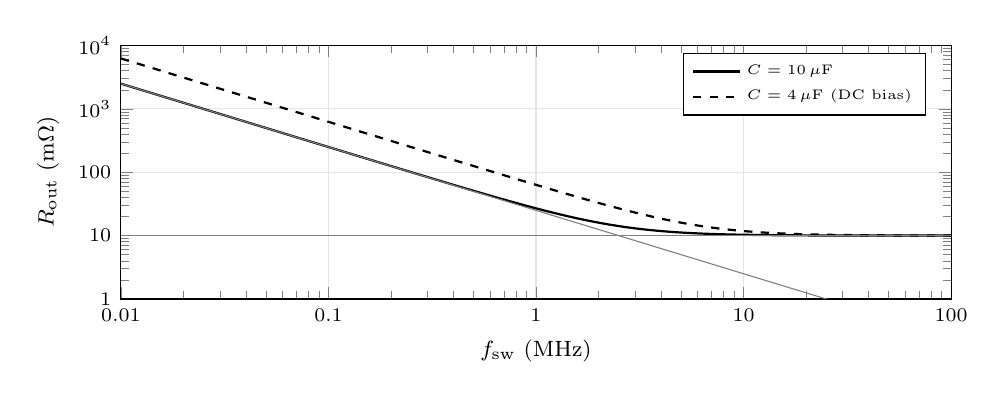
\begin{tikzpicture}
					\begin{loglogaxis}[
							width=\linewidth, height=4.8cm,
							xmin=0.01, xmax=100, ymin=1, ymax=10000,
							xtick={0.01,0.1,1,10,100}, xticklabels={0.01,0.1,1,10,100},
							ytick={1,10,100,1000,10000}, yticklabels={1,10,100,$10^3$,$10^4$},
							xlabel={$f_\mathrm{sw}$ (MHz)}, ylabel={$R_\mathrm{out}$ (m$\Omega$)},
							grid=major, grid style={gray!20},
							tick label style={font=\scriptsize}, label style={font=\footnotesize},
							legend style={font=\tiny, at={(0.97,0.97)}, anchor=north east}, legend cell align=left,
						]
						\addplot[black, thick, domain=-2:2, samples=101] ({10^x}, {sqrt((25/10^x)^2+100)});
						\addlegendentry{$C=10\,\mu$F}
						\addplot[black, thick, dashed, domain=-2:2, samples=101] ({10^x}, {sqrt((62.5/10^x)^2+100)});
						\addlegendentry{$C=4\,\mu$F (DC bias)}
						\addplot[gray, domain=-2:2, samples=2] ({10^x}, {25/10^x});
						\addplot[gray, domain=-2:2, samples=2] ({10^x}, {10});
					\end{loglogaxis}
				\end{tikzpicture}
				\caption{Output resistance of the 2:1 converter, $R_{\mathrm{DS(on)}}=5$\,m$\Omega$ per switch; grey: SSL and FSL asymptotes for $C=10\,\mu$F}
			\end{figure}
		\end{column}
	\end{columns}
	\blfootnote{Source: Seeman and Sanders, 2008 (the square-root combination is an approximation).}
\end{frame}

%%%%%%%%%%%%%%%%%%%%%%%%%%%%%%%%%%%%%%%%%%%%%%%%%%%%%%%%%%%%%
%% Task: R_SSL %%
%%%%%%%%%%%%%%%%%%%%%%%%%%%%%%%%%%%%%%%%%%%%%%%%%%%%%%%%%%%%%
% Two pages: task (page 1) and task with solution (page 2).
\begin{frame}<handout:1-2>
	\frametitle{Output resistance of the 2:1}
	\begin{block}{Task (3 minutes)}
		2:1 converter, $C=10\,\mu$F, $f_\mathrm{sw}=500$\,kHz, $I_\mathrm{out}=10$\,A, $R_{\mathrm{DS(on)}}=5$\,m$\Omega$ per switch.
		\begin{enumerate}
			\item Calculate $R_\mathrm{SSL}$, $R_\mathrm{FSL}$ and $R_\mathrm{out}$.
			\item Loss and output voltage for $V_\mathrm{in}=24$\,V? At which frequency are SSL and FSL equal?
		\end{enumerate}
	\end{block}
	\onslide<2-|handout:2>{
		\begin{enumerate}
			\item $R_\mathrm{SSL}=(1/2)^2/(10\,\mu\mathrm{F}\cdot500\,\mathrm{kHz})=1/(4Cf_\mathrm{sw})=50$\,m$\Omega$; $R_\mathrm{FSL}=2\cdot4\cdot5\,\mathrm{m}\Omega\cdot(1/2)^2=10$\,m$\Omega$; $R_\mathrm{out}\approx51$\,m$\Omega$.
			\item $I^2R_\mathrm{out}=5.1$\,W; $V_\mathrm{out}=12\,\mathrm{V}-0.51\,\mathrm{V}=11.49$\,V, $\eta=95.8$\,\%. Equal at $f_\mathrm{sw}=1/(8R_{\mathrm{DS(on)}}C)=2.5$\,MHz. At 500\,kHz the capacitors dominate.
		\end{enumerate}
	}
\end{frame}

%%%%%%%%%%%%%%%%%%%%%%%%%%%%%%%%%%%%%%%%%%%%%%%%%%%%%%%%%%%%%
%% Task: DC bias %%
%%%%%%%%%%%%%%%%%%%%%%%%%%%%%%%%%%%%%%%%%%%%%%%%%%%%%%%%%%%%%
% Two pages: task (page 1) and task with solution (page 2).
\begin{frame}<handout:1-2>
	\frametitle{The same with DC bias}
	\begin{block}{Task (3 minutes)}
		The 10\,$\mu$F of the flying capacitor are X7R ceramics that lose 60\,\% of their capacitance at 12\,V bias.
		\begin{enumerate}
			\item New $R_\mathrm{SSL}$, loss and efficiency at 10\,A?
			\item Three ways to recover the original 5\,W?
		\end{enumerate}
	\end{block}
	\onslide<2-|handout:2>{
		\begin{enumerate}
			\item $C=4\,\mu$F: $R_\mathrm{SSL}=125$\,m$\Omega$, $R_\mathrm{out}\approx125$\,m$\Omega$: 12.5\,W, $V_\mathrm{out}=10.75$\,V, $\eta=89.6$\,\%.
			\item 2.5 times the nominal capacitance (more parts, or a higher voltage rating that keeps more capacitance); 2.5 times the frequency (1.25\,MHz, still below the FSL corner); soft charging with an inductor, which removes the charge-sharing loss. Always use the capacitance at the operating bias from the data sheet.
		\end{enumerate}
	}
\end{frame}

%%%%%%%%%%%%%%%%%%%%%%%%%%%%%%%%%%%%%%%%%%%%%%%%%%%%%%%%%%%%%
%% Challenge: 3:1 %%
%%%%%%%%%%%%%%%%%%%%%%%%%%%%%%%%%%%%%%%%%%%%%%%%%%%%%%%%%%%%%
% Two pages: challenge (page 1) and solution (page 2).
\begin{frame}<handout:1-2>
	\frametitle{Charge vectors of a 3:1}
	\begin{block}{Challenge (3 minutes)}
		3:1 series-parallel converter with flying capacitors $C_1$, $C_2$: in phase 1 input, $C_1$, $C_2$ and output in series; in phase 2 each capacitor in parallel with the output. Derive $a_\mathrm{c}$ and $R_\mathrm{SSL}$ for $C_1=C_2=C$.
	\end{block}
	\onslide<2-|handout:2>{
		\small
		Phase 1: the same charge $q$ passes input, $C_1$, $C_2$ and output. Phase 2: each capacitor returns $q$ to the output. Output charge per period $q+2q=3q=q_\mathrm{out}$:
		\begin{equation*}
			a_\mathrm{c}=\left(\tfrac13,\tfrac13\right),\qquad q_\mathrm{in}=\tfrac13q_\mathrm{out},\qquad R_\mathrm{SSL}=\frac{2}{9Cf_\mathrm{sw}}
		\end{equation*}
		All seven switches carry $\tfrac13q_\mathrm{out}$. The input switch and the two phase-2 switches of $C_1$ block $2V_\mathrm{out}$, the other four $V_\mathrm{out}$. Both capacitors see $V_\mathrm{out}$.
	}
\end{frame}

%%%%%%%%%%%%%%%%%%%%%%%%%%%%%%%%%%%%%%%%%%%%%%%%%%%%%%%%%%%%%
%% Topologies %%
%%%%%%%%%%%%%%%%%%%%%%%%%%%%%%%%%%%%%%%%%%%%%%%%%%%%%%%%%%%%%
\subsection{Topologies and metrics}

\begin{frame}
	\frametitle{Four 4:1 topologies}
	\begin{table}
		\centering
		\footnotesize
		\begin{tabular}{|l|c|c|c|c|c|c|}
			\hline
			                  & caps & switches & capacitor voltages ($V_\mathrm{out}$) & $\sum a_\mathrm{c}v_\mathrm{c}$ & $\sum a_\mathrm{r}v_\mathrm{r}$ & $\sum a_\mathrm{c}^2$ \\
			\hline
			series-parallel   & 3    & 10       & 1, 1, 1                               & 0.75                            & 4.5                             & 0.19                  \\
			Dickson           & 3    & 8        & 1, 2, 3                               & 1.5                             & 3.0                             & 0.19                  \\
			ladder            & 5    & 8        & all 1                                 & 2.25                            & 3.0                             & 1.19                  \\
			two 2:1 in series & 3    & 8        & 2, 2, 1                               & 1.5                             & 4.0                             & 0.38                  \\
			\hline
		\end{tabular}
		\caption{Charge multipliers of 4:1 step-down converters. $v_\mathrm{c}$, $v_\mathrm{r}$: voltage of each capacitor or (blocked by each) switch in units of $V_\mathrm{out}$, so the sums are in units of $P_\mathrm{out}$; the cascade includes its intermediate capacitor}
	\end{table}
	\small
	\begin{itemize}
		\item $\sum a_\mathrm{c}v_\mathrm{c}$ measures the capacitor energy needed for a given $R_\mathrm{SSL}$, $\sum a_\mathrm{r}v_\mathrm{r}$ the switch area needed for a given $R_\mathrm{FSL}$ (switch VA): lower is better.
		\item Series-parallel is best in capacitors and worst in switches; the ladder the opposite. Dickson combines low capacitor charge with low switch VA.
	\end{itemize}
	\blfootnote{Computed from the topology with the method of Seeman and Sanders, 2008 (\texttt{sc\_analyser.py}, Tutorial 11).}
\end{frame}

%%%%%%%%%%%%%%%%%%%%%%%%%%%%%%%%%%%%%%%%%%%%%%%%%%%%%%%%%%%%%
%% Poll: switch VA %%
%%%%%%%%%%%%%%%%%%%%%%%%%%%%%%%%%%%%%%%%%%%%%%%%%%%%%%%%%%%%%
% Two pages: question (page 1) and answer (page 2).
\begin{frame}<handout:1-2>
	\frametitle{Which needs the most switch VA?}
	\begin{columns}[T]
		\begin{column}{0.48\textwidth}
			\small
			Poll: rank the four 4:1 topologies by total switch VA $\sum a_\mathrm{r}v_\mathrm{r}$, from the lowest to the highest.
			\begin{enumerate}[A]
				\item series-parallel, cascade, Dickson, ladder
				\item ladder and Dickson, cascade, series-parallel
				\item Dickson, series-parallel, ladder, cascade
				\item all equal: the output power is the same
			\end{enumerate}
		\end{column}
		\begin{column}{0.48\textwidth}
			\onslide<2-|handout:2>{
				\begin{block}{Answer: B}
					Ladder and Dickson 3.0, cascade 4.0, series-parallel 4.5 (in $P_\mathrm{out}$). In the series-parallel converter some switches block $3V_\mathrm{out}$ while carrying the same charge as the others; in the ladder every switch blocks only $V_\mathrm{out}$, but the ladder needs the most capacitor energy.
				\end{block}
			}
		\end{column}
	\end{columns}
\end{frame}

%%%%%%%%%%%%%%%%%%%%%%%%%%%%%%%%%%%%%%%%%%%%%%%%%%%%%%%%%%%%%
%% Integrated SC %%
%%%%%%%%%%%%%%%%%%%%%%%%%%%%%%%%%%%%%%%%%%%%%%%%%%%%%%%%%%%%%
\begin{frame}
	\frametitle{Integrated SC converters}
	\begin{columns}[T]
		\begin{column}{0.48\textwidth}
			\small
			\begin{itemize}
				\item On-chip capacitors (MOS, metal--insulator--metal, deep trench) have a parasitic capacitance $\alpha C$ from their bottom plate to the substrate.
				\item It is charged and discharged every period by the swing $v_\mathrm{bp}$ of the bottom plate:
				\begin{equation*}
					P_\mathrm{bp}=\sum_i\alpha_iC_iv_{\mathrm{bp},i}^2f_\mathrm{sw}
				\end{equation*}
				\item The gate charge of the switches adds $\sum Q_\mathrm{G}V_\mathrm{G}f_\mathrm{sw}$ (L4).
			\end{itemize}
		\end{column}
		\begin{column}{0.48\textwidth}
			\small
			\begin{itemize}
				\item $R_\mathrm{SSL}$ falls with $f_\mathrm{sw}$, parasitic and gate losses rise with $f_\mathrm{sw}$: an optimum frequency exists for every load.
				\item At light load the frequency is lowered with the load, so that the efficiency stays flat over decades of current.
				\item Topologies whose flying capacitors swing little at the bottom plate are preferred on chip.
			\end{itemize}
		\end{column}
	\end{columns}
	\blfootnote{Source: Seeman, Ph.D.\ thesis, 2009.}
\end{frame}

%%%%%%%%%%%%%%%%%%%%%%%%%%%%%%%%%%%%%%%%%%%%%%%%%%%%%%%%%%%%%
%% Soft charging %%
%%%%%%%%%%%%%%%%%%%%%%%%%%%%%%%%%%%%%%%%%%%%%%%%%%%%%%%%%%%%%
\subsection{Soft charging and hybrids}

\begin{frame}
	\frametitle{Soft charging}
	\begin{columns}[T]
		\begin{column}{0.5\textwidth}
			\small
			The charge-sharing loss arises when a capacitor meets a voltage source with a different voltage. It disappears if the capacitors are charged by a current source. Two requirements:
			\begin{enumerate}
				\item The SC network feeds a current-source load whose voltage may jump at the phase transitions: an inductor, e.g.\ the input of a buck stage.
				\item No voltage mismatch inside the flying-capacitor network at the transitions. The series-parallel converter fulfils it; other topologies must be checked, some need equal capacitances.
			\end{enumerate}
		\end{column}
		\begin{column}{0.47\textwidth}
			\small
			\begin{itemize}
				\item The capacitors may then ripple more, so less capacitance suffices; the limits are the voltage stress and the swing the inductive stage tolerates.
				\item Example: the Mini-LEGO (L11) uses the inductors of its buck stage to charge the flying capacitors of its 2:1 units softly.
				\item The remaining losses are those of the FSL: switch and ESR conduction.
			\end{itemize}
			\begin{block}{Key message}
				Soft charging turns the $\tfrac12C\Delta V^2$ loss into recovered energy.
			\end{block}
		\end{column}
	\end{columns}
	\blfootnote{Source: Y. Lei, R.\,C.\,N. Pilawa-Podgurski, IEEE Trans.\ Power Electron., vol.\ 30, no.\ 10, 2015.}
\end{frame}

%%%%%%%%%%%%%%%%%%%%%%%%%%%%%%%%%%%%%%%%%%%%%%%%%%%%%%%%%%%%%
%% Resonant SC %%
%%%%%%%%%%%%%%%%%%%%%%%%%%%%%%%%%%%%%%%%%%%%%%%%%%%%%%%%%%%%%
\begin{frame}
	\frametitle{Resonant SC converter}
	\begin{columns}[T]
		\begin{column}{0.5\textwidth}
			\begin{figure}
				\centering
				\begin{circuitikz}[scale=0.62, transform shape]
					\draw (0,0) to[V, l=$V_\mathrm{in}$] (0,7.2) -- (2,7.2) to[nos, l_=(1)] (2,5.6) node[circ]{} coordinate (a);
					\draw (a) -- (2,5.2) to[L, l_=$L_\mathrm{r}$] (2,3.6) -- (2,3.4) to[C, l_=$C$] (2,2.2) -- (2,2.0) node[circ]{} coordinate (b);
					\draw (b) to[nos, l_=(2)] (2,0.4) -- (2,0) -- (0,0);
					\draw (a) to[nos, l=(2)] (4.6,5.6) node[circ]{} coordinate (o);
					\draw (b) to[nos, l_=(1)] (4.6,2.0) -- (o);
					\draw (o) -- (6.0,5.6) to[C, l=$C_\mathrm{o}$] (6.0,0) -- (2,0);
					\draw (6.0,5.6) -- (7.4,5.6) to[R, l=$R_\mathrm{L}$] (7.4,0) -- (6.0,0);
				\end{circuitikz}
				\caption{2:1 resonant SC: a small $L_\mathrm{r}$ in series with $C$; (1), (2): phase in which the switch is closed}
			\end{figure}
		\end{column}
		\begin{column}{0.47\textwidth}
			\footnotesize
			\begin{itemize}
				\item In each phase $L_\mathrm{r}$ and $C$ form a series tank; switching at $f_\mathrm{r}=1/(2\pi\sqrt{L_\mathrm{r}C})$ gives half-sine currents and zero-current switching (ZCS).
				\item 10\,$\mu$F at 500\,kHz: $L_\mathrm{r}=10$\,nH, little more than the layout.
				\item The output receives a rectified sine: peak $\tfrac{\pi}{2}I_\mathrm{out}$, rms per switch $\tfrac{\pi}{4}I_\mathrm{out}$ instead of $0.71\,I_\mathrm{out}$ with constant currents (FSL): the conduction loss is $\pi^2/8=1.23$ times that of the FSL.
				\item No charge-sharing loss. Exactly at $f_\mathrm{r}$ the current is zero at the transitions: ZCS, but no current to charge $C_\mathrm{oss}$; slightly above $f_\mathrm{r}$ a small current remains for ZVS.
			\end{itemize}
		\end{column}
	\end{columns}
	\blfootnote{Source: Lei and Pilawa-Podgurski, 2015 (resonant and soft-charging operation are closely related).}
\end{frame}

%%%%%%%%%%%%%%%%%%%%%%%%%%%%%%%%%%%%%%%%%%%%%%%%%%%%%%%%%%%%%
%% FCML %%
%%%%%%%%%%%%%%%%%%%%%%%%%%%%%%%%%%%%%%%%%%%%%%%%%%%%%%%%%%%%%
\begin{frame}
	\frametitle{Flying-capacitor multilevel converter}
	\begin{columns}[T]
		\begin{column}{0.45\textwidth}
			\begin{figure}
				\centering
				\begin{circuitikz}[scale=0.7, transform shape]
					\draw (-2.4,0) to[V, l=$V_\mathrm{in}$] (-2.4,6.4) -- (1.4,6.4) node[nigfete, anchor=D] (Q1) {};
					\draw (Q1.S) node[circ]{} coordinate (f1);
					\draw (f1) node[nigfete, anchor=D] (Q2) {};
					\draw (Q2.S) node[circ]{} coordinate (sw);
					\draw (sw) node[nigfete, anchor=D] (Q3) {};
					\draw (Q3.S) node[circ]{} coordinate (f2);
					\draw (f2) node[nigfete, anchor=D] (Q4) {};
					\draw (Q4.S) -- (Q4.S |- 0,0) -- (-2.4,0);
					\draw (f1) -- (0.1,0 |- f1) to[C, l_=$C_\mathrm{fly}$] (0.1,0 |- f2) -- (f2);
					\draw (sw) to[L, l=$L$] (4.2,0 |- sw) node[circ]{} coordinate (o);
					\draw (o) to[C, l=$C_\mathrm{o}$] (4.2,0) -- (Q4.S |- 0,0);
					\draw (o) -- (5.4,0 |- sw) to[R, l=$R_\mathrm{L}$] (5.4,0) -- (4.2,0);
					\foreach \q/\n in {Q1/1, Q2/2, Q3/3, Q4/4} \node[anchor=west] at ($(\q.D)!0.5!(\q.S)+(0.3,0)$) {$Q_\n$};
					\node[anchor=north west, font=\footnotesize] at (sw) {switch node};
				\end{circuitikz}
				\caption{Three-level flying-capacitor buck; $Q_1$ to $Q_4$ in series, switch node between $Q_2$ and $Q_3$}
			\end{figure}
		\end{column}
		\begin{column}{0.52\textwidth}
			\footnotesize
			\begin{itemize}
				\item $C_\mathrm{fly}$ is held at $V_\mathrm{in}/2$. The complementary pairs $Q_1/Q_4$ and $Q_2/Q_3$ are driven by PWM signals shifted by half a period.
				\item Every switch blocks $V_\mathrm{in}/2$; the switch node steps by $V_\mathrm{in}/2$ at twice $f_\mathrm{sw}$.
				\item $N$ levels: steps of $V_\mathrm{in}/(N-1)$ at $(N-1)f_\mathrm{sw}$, so the inductance for a given ripple falls with $(N-1)^2$.
				\item The flying-capacitor voltages must stay balanced: natural balancing by the PWM, supported by control.
				\item Example: a six-level GaN flying-capacitor multilevel (FCML) charger for a 400\,V battery uses 100 to 200\,V transistors.
			\end{itemize}
		\end{column}
	\end{columns}
	\blfootnote{Source: R.\,K. Iyer et al., in Kizilyalli et al.\ (eds.), \textit{Wide Bandgap Power Electronics}, Springer, 2025, ch.\ 8.}
\end{frame}

%%%%%%%%%%%%%%%%%%%%%%%%%%%%%%%%%%%%%%%%%%%%%%%%%%%%%%%%%%%%%
%% Hybrid families %%
%%%%%%%%%%%%%%%%%%%%%%%%%%%%%%%%%%%%%%%%%%%%%%%%%%%%%%%%%%%%%
\begin{frame}
	\frametitle{Hybrid converter families}
	\begin{table}
		\centering
		\scriptsize
		\begin{tabular}{|l|>{\raggedright\arraybackslash}p{4.1cm}|>{\raggedright\arraybackslash}p{5.4cm}|}
			\hline
			\textbf{Family}                 & \textbf{Principle}                                                  & \textbf{Typical use}                                                    \\
			\hline
			SC stage plus buck              & SC divides the voltage, the buck regulates and charges softly        & 48\,V to point of load (Mini-LEGO: 48 to 8\,V, then 1\,V)               \\
			Dickson-buck, series-capacitor buck & capacitors in the switching cell of a multiphase buck          & large step-down ratios with low-voltage switches                       \\
			flying-capacitor multilevel     & PWM with balanced flying capacitors                                  & PFC and chargers at 400 to 800\,V with low-voltage GaN                  \\
			resonant SC                     & small inductor per flying capacitor, ZCS                             & fixed-ratio bus converters                                             \\
			diode-capacitor ladders         & multiplier with an inductive input stage                             & high-voltage supplies: $\pm5$\,kV, 2.6\,kW, 95\,\% with 1.7\,kV SiC     \\
			differential power processing   & only the mismatch between stacked loads is converted                 & series-stacked processors in data centres                              \\
			\hline
		\end{tabular}
		\caption{Hybrid switched-capacitor converters}
	\end{table}
	\blfootnote{Sources: Elasser et al., APEC 2023; Kizilyalli et al.\ (eds.), 2025: ch.\ 8 (Iyer et al.), ch.\ 12 (J.\,C. Neely et al.), ch.\ 17 (P. Wang et al.).}
\end{frame}

%%%%%%%%%%%%%%%%%%%%%%%%%%%%%%%%%%%%%%%%%%%%%%%%%%%%%%%%%%%%%
%% Capacitors %%
%%%%%%%%%%%%%%%%%%%%%%%%%%%%%%%%%%%%%%%%%%%%%%%%%%%%%%%%%%%%%
\subsection{Capacitors and regulation}

\begin{frame}
	\frametitle{Capacitors for SC converters}
	\begin{columns}[T]
		\begin{column}{0.48\textwidth}
			\small
			\textbf{Class II MLCC (X5R, X7R)}
			\begin{itemize}
				\item Highest density, but the capacitance falls with DC bias (often by half or more at the rated voltage), with temperature and with age.
				\item Use the data-sheet curve at the operating bias; $R_\mathrm{SSL}$ scales with $1/C_\mathrm{eff}$.
				\item Piezoelectric: audible noise under burst operation.
			\end{itemize}
			\textbf{Class I (C0G)}
			\begin{itemize}
				\item Stable and low-loss: the choice for resonant SC, where $C$ sets $f_\mathrm{r}$ (L9, L10).
			\end{itemize}
		\end{column}
		\begin{column}{0.48\textwidth}
			\small
			\textbf{Layout}
			\begin{itemize}
				\item The ESL and the loop inductance ring with $C$ and limit the current slope: use several small capacitors in parallel, close to the switches (L3).
				\item In resonant SC the loop inductance is part of $L_\mathrm{r}$.
			\end{itemize}
			\textbf{Silicon and deep-trench capacitors}
			\begin{itemize}
				\item Stable over bias and temperature, thin, integrable; lower capacitance per volume than class II MLCC.
			\end{itemize}
		\end{column}
	\end{columns}
\end{frame}

%%%%%%%%%%%%%%%%%%%%%%%%%%%%%%%%%%%%%%%%%%%%%%%%%%%%%%%%%%%%%
%% Regulation %%
%%%%%%%%%%%%%%%%%%%%%%%%%%%%%%%%%%%%%%%%%%%%%%%%%%%%%%%%%%%%%
\begin{frame}
	\frametitle{Regulation}
	\begin{columns}[T]
		\begin{column}{0.48\textwidth}
			\small
			\textbf{Pure SC}
			\begin{itemize}
				\item Frequency modulation: a lower $f_\mathrm{sw}$ raises $R_\mathrm{SSL}$ and lowers $V_\mathrm{out}$; the efficiency stays $V_\mathrm{out}/(V_\mathrm{in}/n)$.
				\item Conductance modulation: in the FSL, a lower gate drive raises the switch resistance.
				\item Reconfigurable topologies switch between ratios (e.g.\ 2:1 and 3:2) to stay close to the ideal ratio.
			\end{itemize}
		\end{column}
		\begin{column}{0.48\textwidth}
			\small
			\textbf{Hybrids}
			\begin{itemize}
				\item PWM of the inductive stage regulates without the linear-regulator penalty, and charges the capacitors softly.
				\item Resonant SC: fixed ratio at $f_\mathrm{r}$; a slight frequency shift tunes ZVS, not the output.
				\item Flying-capacitor balancing: deviations change the switch voltages and the inductor ripple; measure them or control the phase timing.
			\end{itemize}
		\end{column}
	\end{columns}
	\begin{block}{Key message}
		Use the SC stage at its ideal ratio and let an inductor do the regulation.
	\end{block}
\end{frame}

%%%%%%%%%%%%%%%%%%%%%%%%%%%%%%%%%%%%%%%%%%%%%%%%%%%%%%%%%%%%%
%% Brief B6 %%
%%%%%%%%%%%%%%%%%%%%%%%%%%%%%%%%%%%%%%%%%%%%%%%%%%%%%%%%%%%%%
\begin{frame}
	\frametitle{Brief B6: 48 to 12\,V}
	\begin{columns}[T]
		\begin{column}{0.48\textwidth}
			\small
			150\,W at 12\,V: $I_\mathrm{out}=12.5$\,A. A budget of 1\,\% for charge sharing allows
			\begin{equation*}
				R_\mathrm{SSL}\leq\frac{1.5\,\mathrm{W}}{(12.5\,\mathrm{A})^2}=9.6\,\mathrm{m}\Omega
			\end{equation*}
			4:1 series-parallel or Dickson, $\sum a_\mathrm{c}^2=3/16$, equal capacitors:
			\begin{equation*}
				Cf_\mathrm{sw}\geq\frac{3/16}{9.6\,\mathrm{m}\Omega}=19.5\,\mathrm{F/s}
			\end{equation*}
			At 1\,MHz: 19.5\,$\mu$F effective per flying capacitor; with 60\,\% derating about 49\,$\mu$F nominal.
		\end{column}
		\begin{column}{0.48\textwidth}
			\small
			\begin{itemize}
				\item Series-parallel: all capacitors at 12\,V, but switches up to 36\,V. Dickson: capacitors at 12, 24 and 36\,V, switches at 12 and 24\,V.
				\item The 36\,V capacitor of the Dickson loses more capacitance under bias: compare the data sheets.
				\item Soft charging with a small inductor (resonant or hybrid) removes the SSL budget and leaves the FSL: then the switches decide.
				\item The choice enters the layout and the bill of materials of milestone M3 (20.01.).
			\end{itemize}
		\end{column}
	\end{columns}
\end{frame}

%%%%%%%%%%%%%%%%%%%%%%%%%%%%%%%%%%%%%%%%%%%%%%%%%%%%%%%%%%%%%
%% Key messages %%
%%%%%%%%%%%%%%%%%%%%%%%%%%%%%%%%%%%%%%%%%%%%%%%%%%%%%%%%%%%%%
\begin{frame}
	\frametitle{Key messages}
	\begin{enumerate}
		\item An SC converter is an ideal $n$:1 transformer with an output resistance; efficiency $V_\mathrm{out}/(V_\mathrm{in}/n)$.
		\item Charging a capacitor from a voltage source loses $\tfrac12C\Delta V^2$, independent of the resistance.
		\item Charge-multiplier vectors follow from the topology; $R_\mathrm{SSL}=\sum a_\mathrm{c}^2/(Cf_\mathrm{sw})$, $R_\mathrm{FSL}=2\sum Ra_\mathrm{r}^2$.
		\item Topologies trade capacitor energy against switch VA: series-parallel and ladder are the extremes.
		\item DC bias can halve the capacitance and double $R_\mathrm{SSL}$: design with the effective value.
		\item Soft charging, resonant SC and hybrids remove the charging loss; the inductor regulates.
	\end{enumerate}
\end{frame}

%%%%%%%%%%%%%%%%%%%%%%%%%%%%%%%%%%%%%%%%%%%%%%%%%%%%%%%%%%%%%
%% Exit ticket %%
%%%%%%%%%%%%%%%%%%%%%%%%%%%%%%%%%%%%%%%%%%%%%%%%%%%%%%%%%%%%%
% Two pages: questions (page 1) and answers (page 2).
\begin{frame}<handout:1-2>
	\frametitle{Exit questions}
	\begin{varblock}[\textwidth]{Three questions, one minute each}
		\begin{enumerate}
			\item A 3:1 series-parallel converter uses 22\,$\mu$F per flying capacitor at 250\,kHz. Calculate $R_\mathrm{SSL}$.
			\item Why does a smaller switch resistance not reduce the charge-sharing loss?
			\item A 2:1 converter delivers 5.6\,V from 12\,V. What is its highest possible efficiency?
		\end{enumerate}
	\end{varblock}
	\onslide<2-|handout:2>{
		\begin{enumerate}
			\item $R_\mathrm{SSL}=2/(9\cdot22\,\mu\mathrm{F}\cdot250\,\mathrm{kHz})=40$\,m$\Omega$.
			\item The loss $\tfrac12C\Delta V^2$ follows from the energy balance alone; the resistance only sets how fast it happens.
			\item $\eta\leq5.6/6=93.3$\,\%.
		\end{enumerate}
	}
\end{frame}

%%%%%%%%%%%%%%%%%%%%%%%%%%%%%%%%%%%%%%%%%%%%%%%%%%%%%%%%%%%%%
%% References %%
%%%%%%%%%%%%%%%%%%%%%%%%%%%%%%%%%%%%%%%%%%%%%%%%%%%%%%%%%%%%%
\begin{frame}
	\frametitle{References}
	\scriptsize
	\begin{itemize}
		\item M.\,D. Seeman, S.\,R. Sanders, ``Analysis and optimization of switched-capacitor DC-DC converters,'' IEEE Trans.\ Power Electron., vol.\ 23, no.\ 2, pp.\ 841--851, 2008.
		\item M.\,D. Seeman, ``A design methodology for switched-capacitor DC-DC converters,'' Ph.D.\ dissertation, UC Berkeley, Tech.\ Rep.\ UCB/EECS-2009-78, 2009.
		\item Y. Lei, R.\,C.\,N. Pilawa-Podgurski, ``A general method for analyzing resonant and soft-charging operation of switched-capacitor converters,'' IEEE Trans.\ Power Electron., vol.\ 30, no.\ 10, pp.\ 5650--5664, 2015.
		\item J.\,G. Kassakian, D.\,J. Perreault, G.\,C. Verghese, M.\,F. Schlecht, \textit{Principles of Power Electronics}, 2nd ed., Cambridge University Press, 2023.
		\item I.\,C. Kizilyalli, Z.\,J. Shen, D.\,W. Cunningham (eds.), \textit{Wide Bandgap Power Electronics}, Springer, 2025: ch.\ 8 (R.\,K. Iyer et al., FCML for EV charging), ch.\ 12 (J.\,C. Neely et al., hybrid SC at medium voltage), ch.\ 17 (P. Wang, M. Chen, R. Pilawa-Podgurski, differential power processing).
		\item Y. Elasser et al., ``Mini-LEGO: a 1.5-MHz 240-A 48-V-to-1-V CPU VRM with 8.4-mm height for vertical power delivery,'' IEEE APEC 2023.
		\item D.\,J. Perreault, MIT 6.622 Power Electronics, Lectures 31 and 32 (switched-capacitor converters), 2023.
	\end{itemize}
\end{frame}
